\documentclass[10pt, unknownkeysallowed]{beamer}

% Theme
\usetheme[numbering = fraction, progressbar=frametitle]{metropolis} 

%\useoutertheme{shadow} % Alternatively: infolines, miniframes, shadow, sidebar, smoothbars, smoothtree, split, tree
\useinnertheme{rectangles} % Alternatively: rectangles, circles, inmargin, rounded

% Standard Packages
\usepackage{appendixnumberbeamer}

\usepackage[utf8]{inputenc}
\usepackage[ngerman]{babel}

\usepackage{booktabs}
\usepackage[scale=2]{ccicons}

\usepackage{pgfplots}
\usepgfplotslibrary{dateplot}

\usepackage{xspace}
\newcommand{\themename}{\textbf{\textsc{metropolis}}\xspace}

\usepackage{media9}
\usepackage{animate}
\usepackage{graphicx, subfig}
\usepackage[export]{adjustbox}

\usepackage{wrapfig}

\usepackage{floatflt}

\usepackage{tabto}

\usepackage[font=scriptsize, figurename=Abb.]{caption}

% Paths
\graphicspath{{img/}}

%Einstellungen der Präsentationen
\title{Reverse Proxies \& Docker Swarm}
\subtitle{LINUX DAYS VILLACH}
\author[FK]{Florian Kleber}
\institute[HTL-Villach IT]{Höhere technische Bundeslehr- und Versuchsanstalt Villach}
\date{17. Mai 2019}

% Colors
%\definecolor{UBCblue}{rgb}{0.04706, 0.13725, 0.26667} % UBC Blue (primary)
%\definecolor{UBCgrey}{rgb}{0.3686, 0.5255, 0.6235} % UBC Grey (secondary)
%\definecolor{chocolate}{RGB}{33,33,33}

\definecolor{htl-gelb}{RGB}{255,242,51}
\definecolor{htl-schwarz}{RGB}{0,0,0}
\definecolor{royalblue(web)}{rgb}{0.25, 0.41, 0.88}
\definecolor{royalblue(traditional)}{RGB}{10,59,97}

%\setbeamercolor{alerted text}{fg=red}
%\setbeamercolor{background canvas}{bg=white}
%\setbeamercolor{block body alerted}{bg=normal text.bg!90!black}
%\setbeamercolor{block body}{bg=normal text.bg!90!black}
%\setbeamercolor{block body example}{bg=normal text.bg!90!black}
%\setbeamercolor{block title alerted}{use={normal text,alerted text},fg=alerted text.fg!75!normal text.fg,bg=normal text.bg!75!black}
%\setbeamercolor{block title}{bg=blue}
%\setbeamercolor{block title example}{use={normal text,example text},fg=example text.fg!75!normal text.fg,bg=normal text.bg!75!black}
%\setbeamercolor{fine separation line}{}
\setbeamercolor{frametitle}{bg=royalblue(traditional), fg=white}
%\setbeamercolor{item projected}{fg=black}
%\setbeamercolor{normal text}{fg=royalblue(traditional),bg=white}
%\setbeamercolor{palette sidebar primary}{use=normal text,fg=normal text.fg}
%\setbeamercolor{palette sidebar quaternary}{use=structure,fg=structure.fg}
%\setbeamercolor{palette sidebar secondary}{use=structure,fg=structure.fg}
%\setbeamercolor{palette sidebar tertiary}{use=normal text,fg=normal text.fg}
%\setbeamercolor{section in sidebar}{fg=brown}
%\setbeamercolor{section in sidebar shaded}{fg=grey}
%\setbeamercolor{separation line}{}
%\setbeamercolor{sidebar}{bg=red}
%\setbeamercolor{sidebar}{parent=palette primary}
%\setbeamercolor{structure}{bg=white, fg=black}
%\setbeamercolor{subsection in sidebar}{fg=brown}
%\setbeamercolor{subsection in sidebar shaded}{fg=grey}
%\setbeamercolor{title}{fg=brown}
%\setbeamercolor{titlelike}{fg=brown}
%\usepackage{graphicx}
%\usepackage{color}
\usetheme[numbering = fraction, progressbar=frametitle]{metropolis} 


\makeatletter
\newsavebox{\mybox}
\setbeamertemplate{frametitle}{%
  \nointerlineskip%
  \savebox{\mybox}{%
      \begin{beamercolorbox}[%
          wd=\paperwidth,%
          sep=0pt,%
          leftskip=\metropolis@frametitle@padding,%
          rightskip=\metropolis@frametitle@padding,%
        ]{frametitle}%
      \metropolis@frametitlestrut@start\insertframetitle\metropolis@frametitlestrut@end%
      \end{beamercolorbox}%
    }
  \begin{beamercolorbox}[%
      wd=\paperwidth,%
      sep=0pt,%
      leftskip=\metropolis@frametitle@padding,%
      rightskip=\metropolis@frametitle@padding,%
    ]{frametitle}%
  \metropolis@frametitlestrut@start\insertframetitle\metropolis@frametitlestrut@end%
  \hfill%
  \raisebox{-\metropolis@frametitle@padding}{
\includegraphics[height=\dimexpr\ht\mybox+\metropolis@frametitle@padding\relax]{Linuxwochen.png}}%
  ~%
    \hspace*{-3px}
    \raisebox{-\metropolis@frametitle@padding}{
\includegraphics[height=\dimexpr\ht\mybox+\metropolis@frametitle@padding\relax]{HTL-Logo.png}}%
    \hspace*{-\metropolis@frametitle@padding}
    \hspace*{-8px}
  \end{beamercolorbox}%
}

\addtobeamertemplate{frametitle}{}{%
    \usebeamertemplate*{progress bar in head/foot}
}

\makeatother


\begin{document}

\maketitle

\begin{frame}{Agenda}
%\frametitle{Übersicht}
%\frametitle{\rlap{\raisebox{-\dp\strutbox}{
\includegraphics[height=\baselineskip]{HTL-Logo.png}}}Your frame title}
%\setbeamertemplate{section in toc}[sections numbered]
%\vspace*{8pt}
\begin{minipage}{.45\textwidth}
    \tableofcontents[]
\end{minipage}
\hfill
\begin{minipage}{.45\textwidth}
    
\includegraphics[width=\linewidth,center]{LinuxPinguin2.png}
\end{minipage}
%\tableofcontents[hideallsubsections]
\end{frame}

\section{about_me}
\begin{frame}{Über Mich}
\begin{minipage}{.45\textwidth}
	
\includegraphics[width=\linewidth]{chrome_2019-05-17_13-24-38.png}
	\vspace*{-16px}
	\\
\end{minipage}
\hfill\vline\hfill
\begin{minipage}{.45\textwidth}
    \vspace*{-20px}
	\textbf{Qualifikation:}
	\begin{itemize}
	    \item htl J1
		\item htl J2
		\item htl J3
		\item htl J4
	\end{itemize}
	\textbf{Interessen:}
	\begin{itemize}
	    \item Full Stack Developement
		\item github
		\item Linux
		\item systemd
		\item DnD
	\end{itemize}
\end{minipage}
\end{frame}



\section{Motivation}



\begin{frame}{Motivation}
\begin{minipage}{.45\textwidth}
    \vspace*{5px}
    \textbf{Tools:}
	\begin{itemize}
	    \item \textbf{Warum Docker?}
		\item Warum Reverse Proxies?
		\item Warum Docker Swarm?
		\item Warum Cloudflare?
	\end{itemize}
	\vspace*{10px}
    \animategraphics[autoplay,loop,width=\linewidth]{10}{gitforking-}{0}{37}
	\captionof{figure}{
	    \raggedright
		\label{fig:forking}
		Quelle: GitHub, 2016
	}  
\end{minipage}
\hfill\vline\hfill
\begin{minipage}{.45\textwidth}
    \vspace*{15px}
    \textbf{github.com/linux-days-villach}
    
\includegraphics[width=\linewidth,center]{qr-code.png}
	\captionof{figure}{
		\label{fig:QRcode}
	    \\
		Quelle: \\
		QRCode Monkey, Air Quality Monitoring Station, 2018
	}  
\end{minipage}
\end{frame}


\subsection{Warum Docker?}


\begin{frame}{Warum Docker?}
\begin{minipage}{\textwidth}
    \includegraphics[width=\textwidth]{Motivation1.png}
	\captionof{figure}{
		\label{fig:karte2}
		\textbf{\small Anwendungsstacks mit Docker Compose}
		\\
		Quelle: Medieval and Renaissance Maps von Chet Van Duzer
		\vspace*{-8.4px}
		\\
	}   
\end{minipage}
\end{frame}

\begin{frame}{Motivation}
\begin{minipage}{.45\textwidth}
    \vspace*{5px}
    \textbf{Tools:}
	\begin{itemize}
	    \item Warum Docker?
		\item \textbf{Warum Reverse Proxies?}
		\item Warum Docker Swarm?
		\item Warum Cloudflare?
	\end{itemize}
	\vspace*{10px}
    \animategraphics[autoplay,loop,width=\linewidth]{10}{gitforking-}{0}{37}
	\captionof{figure}{
	    \raggedright
		\label{fig:forking}
		Quelle: GitHub, 2016
	}  
\end{minipage}
\hfill\vline\hfill
\begin{minipage}{.45\textwidth}
    \vspace*{15px}
    \textbf{github.com/linux-days-villach}
    
\includegraphics[width=\linewidth,center]{qr-code.png}
	\captionof{figure}{
		\label{fig:QRcode}
	    \\
		Quelle: \\
		QRCode Monkey, Air Quality Monitoring Station, 2018
	}  
\end{minipage}
\end{frame}


\subsection{Warum Reverse Proxies?}


\begin{frame}{Warum Reverse Proxies?}
\begin{minipage}{\textwidth}
    \animategraphics[autoplay,loop,width=\linewidth]{10}{wetterhost-}{0}{45}
	\captionof{figure}{
		\label{fig:karte2}
		\textbf{\small Anwendungsstacks mit Docker Compose}
		\\
		Quelle: Medieval and Renaissance Maps von Chet Van Duzer
		\vspace*{-8.4px}
		\\
	}   
\end{minipage}
\end{frame}

\begin{frame}{Motivation}
\begin{minipage}{.45\textwidth}
    \vspace*{5px}
    \textbf{Tools:}
	\begin{itemize}
	    \item Warum Docker?
		\item Warum Reverse Proxies?
		\item \textbf{Warum Docker Swarm?}
		\item Warum Cloudflare?
	\end{itemize}
	\vspace*{10px}
    \animategraphics[autoplay,loop,width=\linewidth]{10}{gitforking-}{0}{37}
	\captionof{figure}{
	    \raggedright
		\label{fig:forking}
		Quelle: GitHub, 2016
	}  
\end{minipage}
\hfill\vline\hfill
\begin{minipage}{.45\textwidth}
    \vspace*{15px}
    \textbf{github.com/linux-days-villach}
    
\includegraphics[width=\linewidth,center]{qr-code.png}
	\captionof{figure}{
		\label{fig:QRcode}
	    \\
		Quelle: \\
		QRCode Monkey, Air Quality Monitoring Station, 2018
	}  
\end{minipage}
\end{frame}


\subsection{Warum Docker Swarm?}


\begin{frame}{Warum Docker Swarm?}
\begin{minipage}{.45\textwidth}
\captionof{figure}{
        \vspace*{5px}
        \\
        \textbf{\small Erwartete Funktionsweise von Docker Swarm}
        \vspace*{-2px}
        \\
        
\includegraphics[width=\linewidth,center]{Motivation3.png}
		\label{fig:tagesblatt}
		\vspace*{-10px}
		\\
		Quelle: \\
		https://rominirani.com/docker-swarm-tutorial-b67470cf8872
	}  
\end{minipage}
\hfill\vline\hfill
\begin{minipage}{.45\textwidth}
    \vspace*{-10px}
	\textbf{Warum nicht k8s?}
	\begin{itemize}
	    \item Kosten?
	    \item Zielgruppe?
	    \item Wartungsaufwand?
		\item Vefügbarkeit 99ish\%
		\item Lohnt sich ein 3Node k8s?
		\item Warum nicht AWS?
	\end{itemize}
	\textbf{Docker Compose?}
	\begin{itemize}
	    \item Failover?
		\item Webinterface?
		\item Monitoring?
		\item Know-how?
	\end{itemize}
    \vspace*{-10px}
\end{minipage}
\end{frame}

\begin{frame}{Warum Docker Swarm?}
\begin{minipage}{.45\textwidth}
    \vspace*{-36px}
	\textbf{Cool Faktor}
	\begin{itemize}
	    \item Günstig
		\item Einfach
		\item Schnell
		\item Skalierbar
	\end{itemize}
	\textbf{Wozu?}
	\begin{itemize}
	    \item CI/CD
		\item Load Balancing
	\end{itemize}
	\textbf{Wo?}
	\begin{itemize}
	    \item Development
	\end{itemize}
\end{minipage}
\hfill\vline\hfill
\begin{minipage}{.45\textwidth}
	%\captionof{figure}{
	%   \vspace*{5px}
    %    \\
    %    \textbf{\small Vereinfachte Funktionsweise von Docker Swarm}
    %    \vspace*{3px}
    %    \\
    %    \center
    %    \animategraphics[autoplay,loop,height=135px]{40}{betterdockerlogo-}{0}{71}
	%	\label{fig:tagesblatt}
	%    \\
	%	Quelle: \\
	%	https://github.com/NBISweden/LocalEGA-deploy-swarm
	%}
	\begin{figure}
	    \vspace*{5px}
	    \textbf{\raggedright\small Vereinfachte Funktionsweise von Docker Swarm}
	    \vspace*{5px}
	    \\
        \centering
        \animategraphics[autoplay,loop,height=135px]{40}{betterdockerlogo-}{0}{71}
        \label{fig:tagesblatt}
        \caption{
            Quelle: 
            \\	
            https://github.com/NBISweden/LocalEGA-deploy-swarm}
    \end{figure}
\end{minipage}
\end{frame}

\begin{frame}{Motivation}
\begin{minipage}{.45\textwidth}
    \vspace*{5px}
    \textbf{Tools:}
	\begin{itemize}
	    \item Warum Docker?
		\item Warum Reverse Proxies?
		\item Warum Docker Swarm?
		\item \textbf{Warum Cloudflare?}
	\end{itemize}
	\vspace*{10px}
    \animategraphics[autoplay,loop,width=\linewidth]{10}{gitforking-}{0}{37}
	\captionof{figure}{s
	    \raggedright
		\label{fig:forking}
		Quelle: GitHub, 2016
	}  
\end{minipage}
\hfill\vline\hfill
\begin{minipage}{.45\textwidth}
    \vspace*{15px}
    \textbf{github.com/linux-days-villach}
    
\includegraphics[width=\linewidth,center]{qr-code.png}
	\captionof{figure}{
		\label{fig:QRcode}
	    \\
		Quelle: \\
		QRCode Monkey, Air Quality Monitoring Station, 2018
	}  
\end{minipage}
\end{frame}


\subsection{Warum Cloudflare?}


\begin{frame}{Warum Cloudflare?}
\begin{minipage}{\textwidth}
    \vspace*{5px}
    \hfill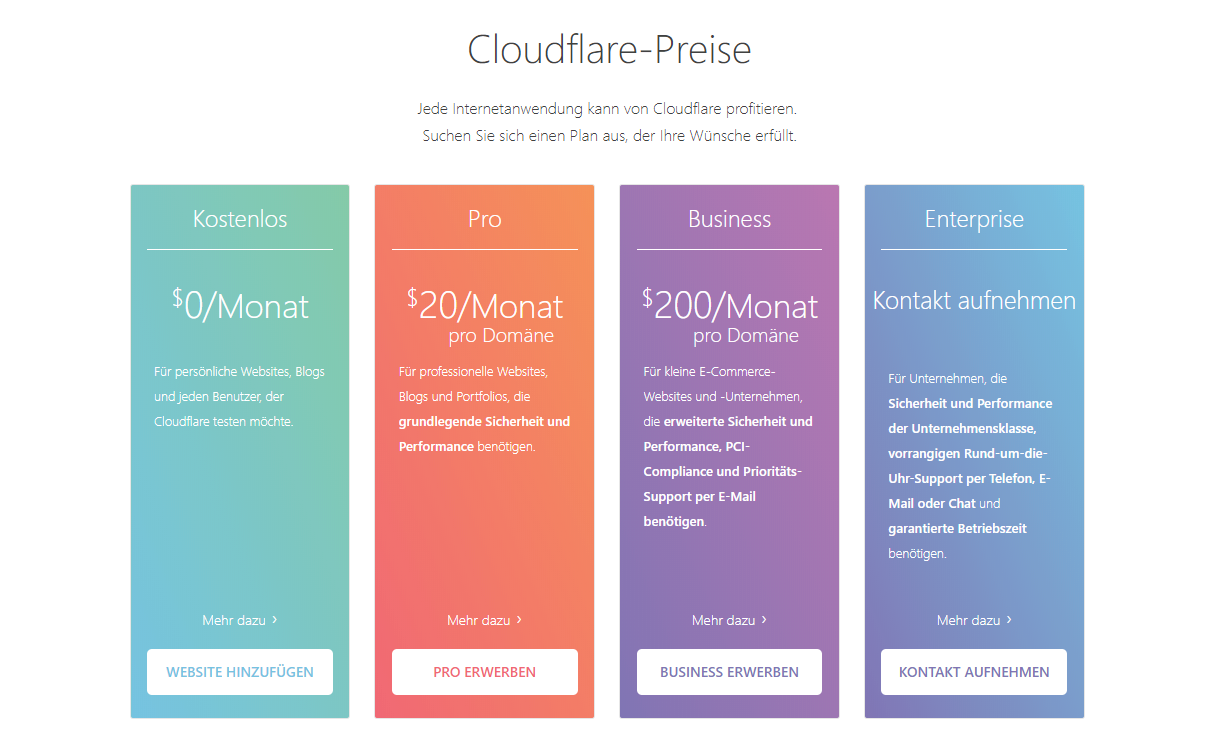
\includegraphics[height=170px]{cloudflare.png}\hfill
    \vspace*{10px}
	\captionof{figure}{
		\label{fig:karte2}
		\raggedright
		\textbf{\small Cloudflare-Preise}
		\\
		Quelle: https://www.cloudflare.com/plans/
		\vspace*{-9px}
		\\
	}   
\end{minipage}
\end{frame}



\section{Optionen}


\subsection{nginx}



\begin{frame}{nginx}
\begin{minipage}{\textwidth}
    \vspace*{10px}
    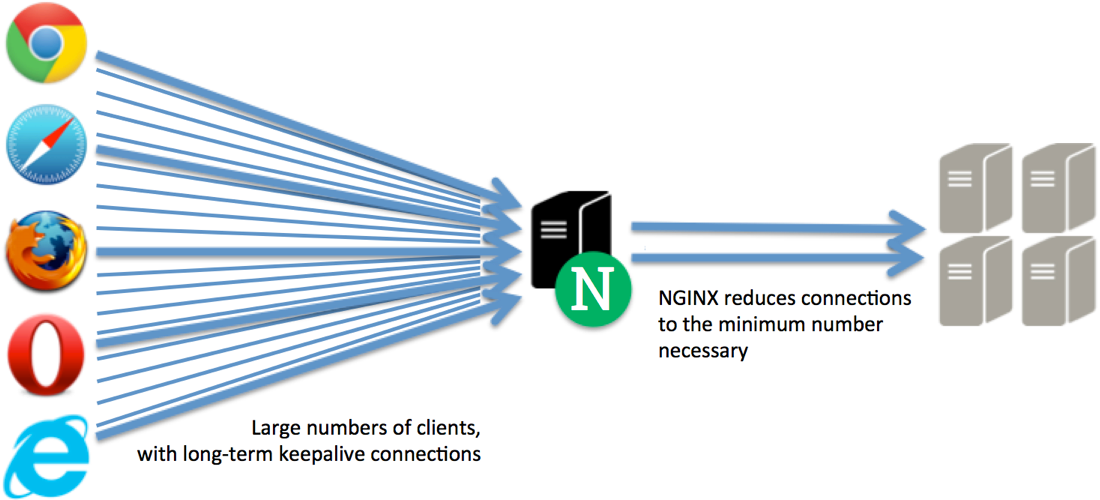
\includegraphics[width=\textwidth]{nginx.png}
    \vspace*{20px}
	\captionof{figure}{
		\label{fig:karte2}
		\textbf{\small Nginx Reverse Proxies}
		\\
		Quelle: https://www.nginx.com/blog/load-balancing-with-nginx-plus-part2/
		\vspace*{-9px}
		\\
	}   
\end{minipage}
\end{frame}


\subsection{envoy}


\begin{frame}{envoy}
\begin{minipage}{\textwidth}
    \vspace*{5px}
    \hfill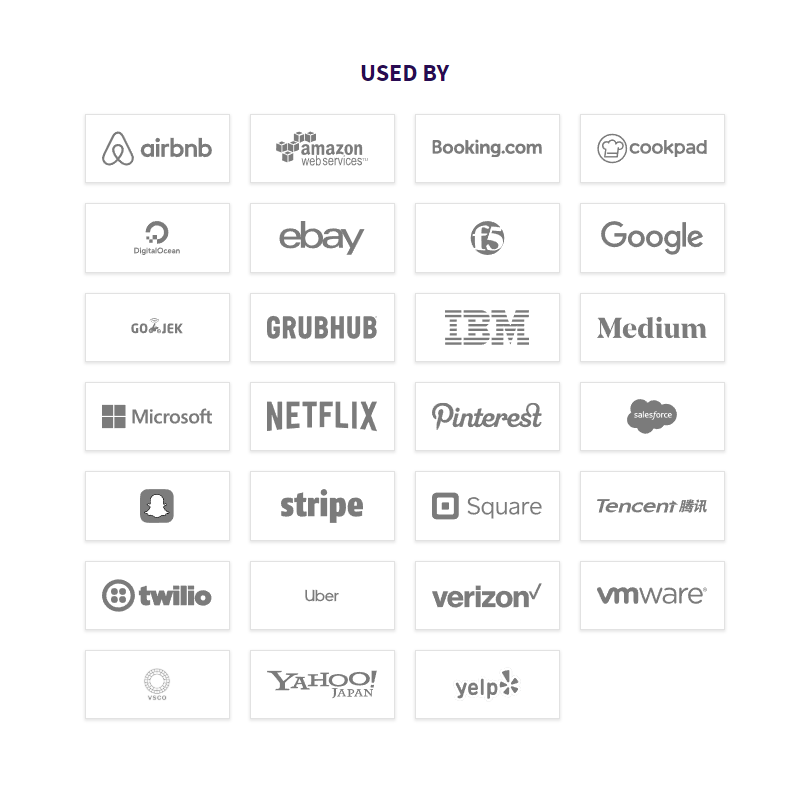
\includegraphics[height=170px]{envoy.png}\hfill
    \vspace*{10px}
	\captionof{figure}{
		\label{fig:karte2}
		\raggedright
		\textbf{\small Envoy Portfolio}
		\\
		Quelle: https://www.envoyproxy.io/
		\vspace*{-9px}
		\\
	}   
\end{minipage}
\end{frame}


\subsection{traefik}


\begin{frame}{traefik}
\begin{minipage}{\textwidth}
    \vspace*{10px}
    \hfill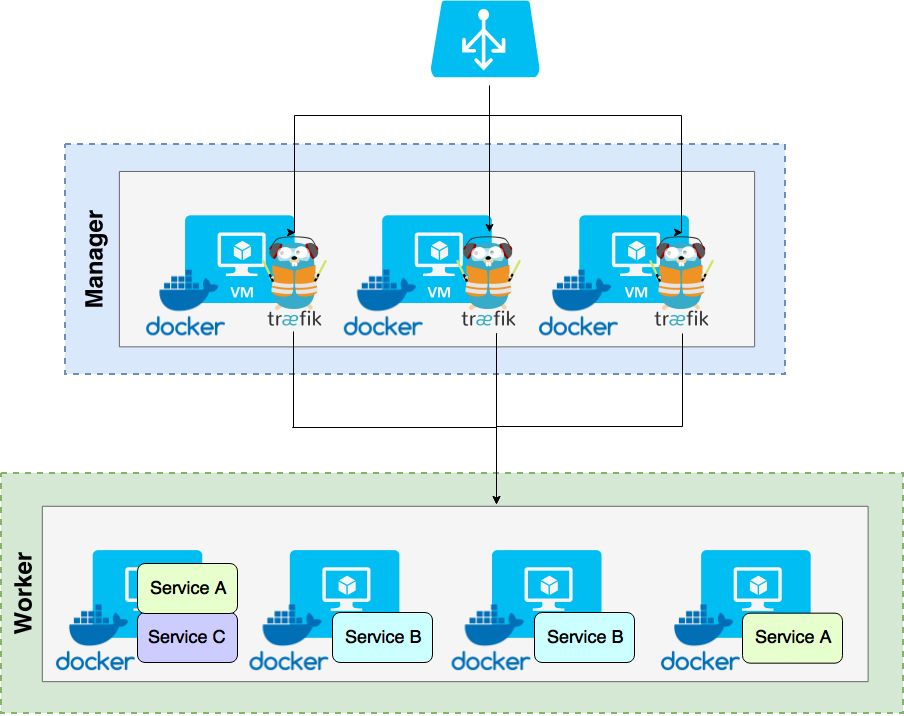
\includegraphics[height=170px]{ha-traefik.png}\hfill
    \vspace*{10px}
	\captionof{figure}{
		\label{fig:karte2}
		\textbf{\small traefik Reverse Proxies}
		\\
		Quelle: https://jmaitrehenry.ca/2017/12/15/using-traefik-with-docker-swarm-and-consul-as-your-load-balancer/
		\vspace*{-9px}
		\\
	}   
\end{minipage}
\end{frame}



\section{Beispiel}



\subsection{Theorie}
\begin{frame}{Theorie}
\begin{minipage}{\textwidth}
    \vspace*{10px}
    \hfill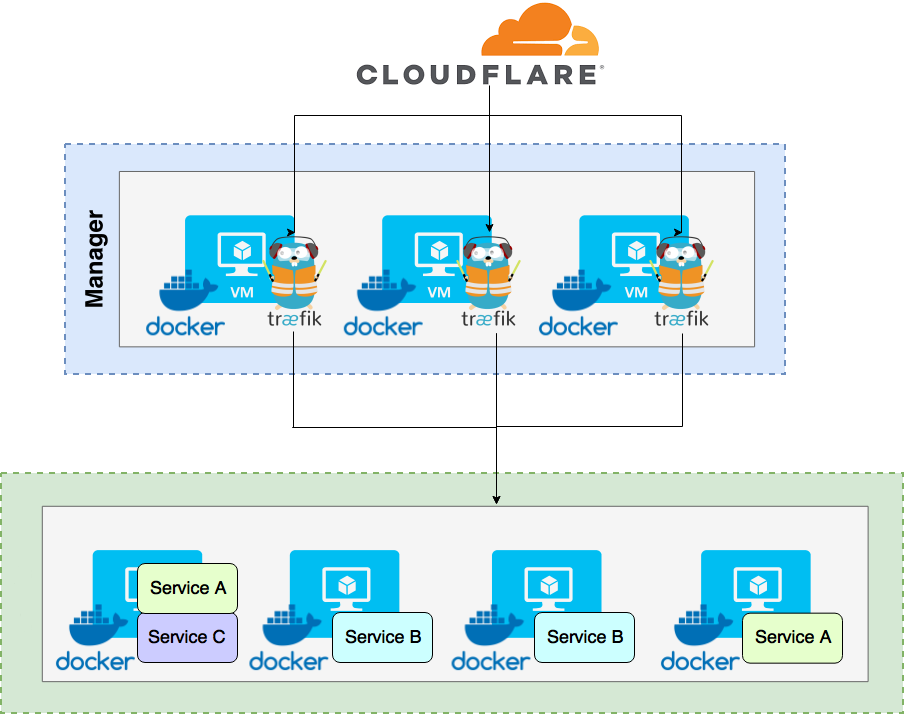
\includegraphics[height=170px]{ha-traefik2.png}\hfill
    \vspace*{10px}
	\captionof{figure}{
		\label{fig:karte2}
		\textbf{\small HA traefik Beispiel}
		\\
		Quelle: https://serverfault.com/questions/919349/how-to-setup-traefik-for-ha-need-a-reverse-proxy-in-front-of-traefik
		\vspace*{-9px}
		\\
	}   
\end{minipage}
\end{frame}

\begin{frame}{Theorie}
\begin{minipage}{\textwidth}
    \animategraphics[autoplay,loop,width=\linewidth]{10}{wetterhost-}{0}{45}
	\captionof{figure}{
		\label{fig:karte2}
		\raggedright
		\textbf{\small HA traefik Beispiel}
		\\
		Quelle: https://docs.traefik.io/basics/#concepts
		\vspace*{-8.4px}
		\\
	}   
\end{minipage}
\end{frame}



\subsection{Praxis}


\begin{frame}{Praxis}
\begin{minipage}{\textwidth}
    \vspace*{10px}
    \hfill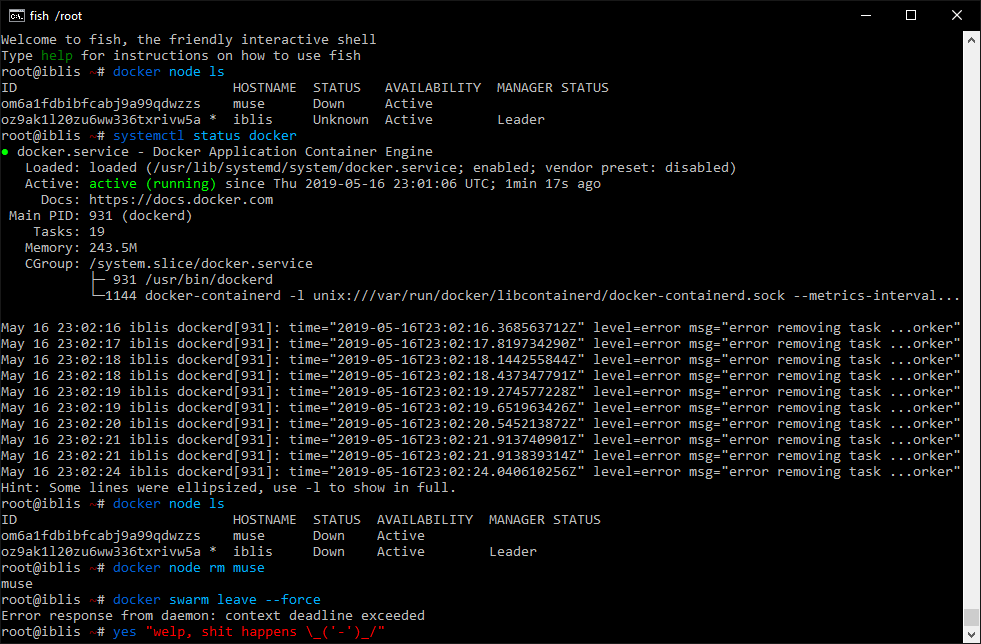
\includegraphics[height=170px]{praxis.png}\hfill
    \vspace*{10px}
	\captionof{figure}{
		\label{fig:karte2}
		\raggedright
		\textbf{\small HA traefik Beispiel}
		\\
		Quelle: Bei mir Daham, Gestan am Obend
		\vspace*{-9px}
		\\
	}   
\end{minipage}
\end{frame}

\begin{frame}{Praxis}
\begin{minipage}{\textwidth}
    \vspace*{10px}
    \hfill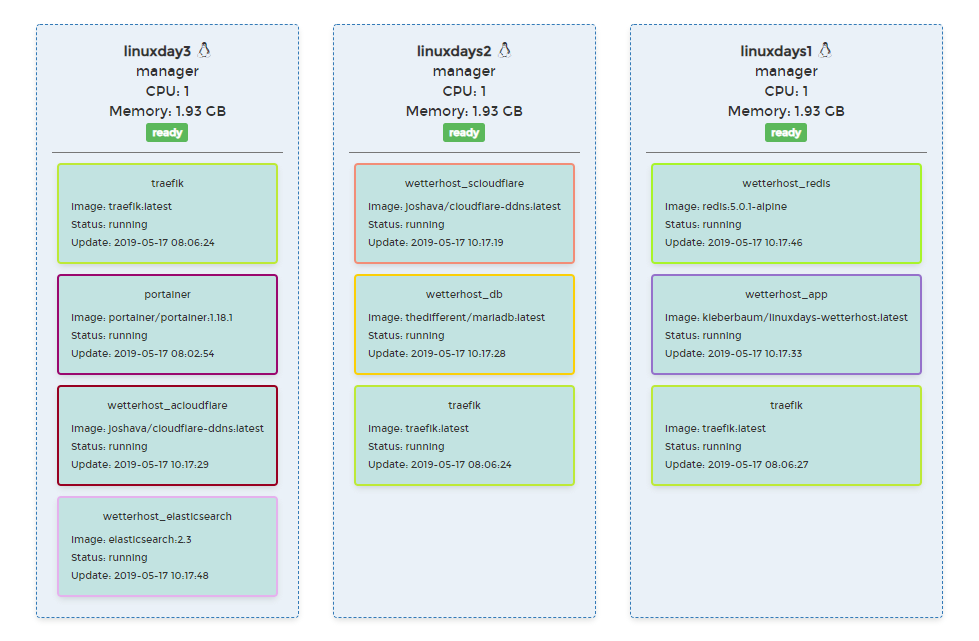
\includegraphics[height=170px]{nodes.png}\hfill
    \vspace*{10px}
	\captionof{figure}{
		\label{fig:karte2}
		\raggedright
		\textbf{\small HA traefik Beispiel}
		\\
		Quelle: Bei mir Daham, Gestan am Obend
		\vspace*{-9px}
		\\
	}   
\end{minipage}
\end{frame}

\begin{frame}{Praxis}
\begin{minipage}{\textwidth}
    \vspace*{10px}
    \hfill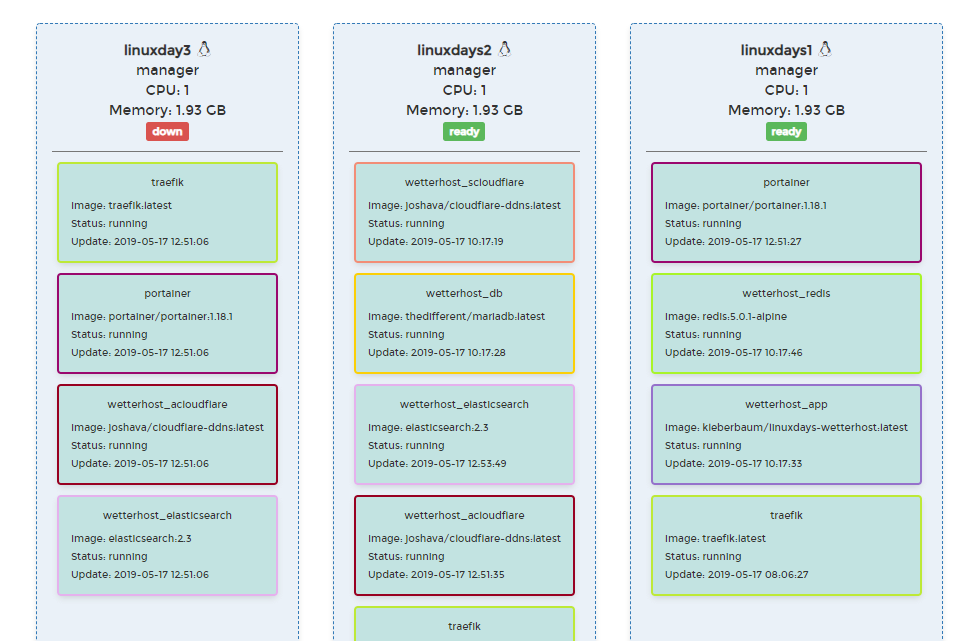
\includegraphics[height=170px]{nodes2.png}\hfill
    \vspace*{10px}
	\captionof{figure}{
		\label{fig:karte2}
		\raggedright
		\textbf{\small HA traefik Beispiel}
		\\
		Quelle: Bei mir Daham, Gestan am Obend
		\vspace*{-9px}
		\\
	}   
\end{minipage}
\end{frame}

\begin{frame}{Praxis}
\begin{minipage}{\textwidth}
    \vspace*{10px}
    \hfill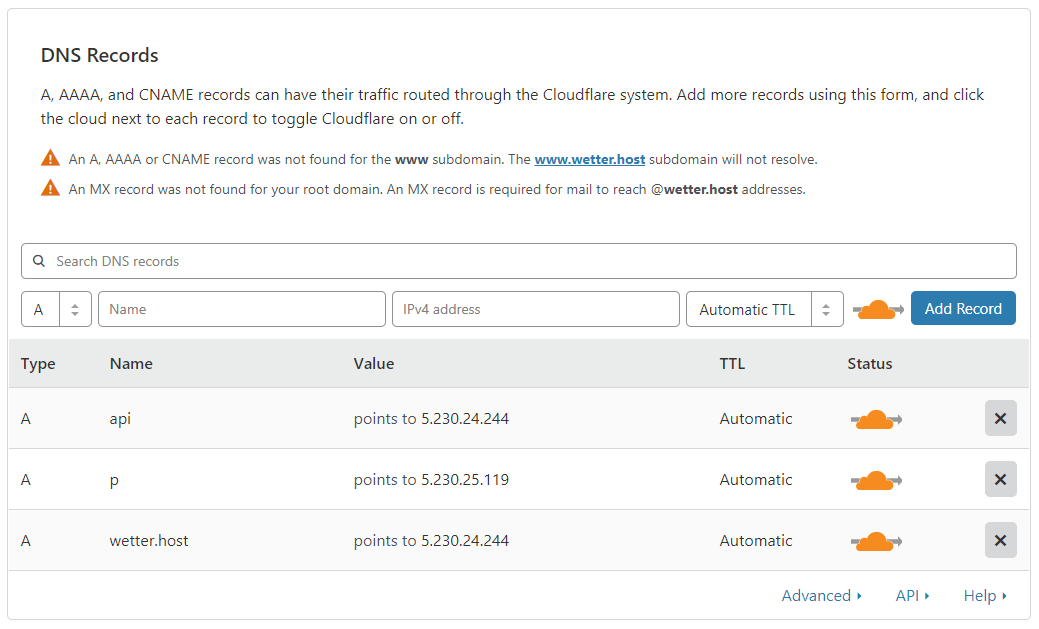
\includegraphics[height=170px]{demo1.png}\hfill
    \vspace*{10px}
	\captionof{figure}{
		\label{fig:karte2}
		\raggedright
		\textbf{\small HA traefik Beispiel}
		\\
		Quelle: Bei mir Daham, Gestan am Obend
		\vspace*{-9px}
		\\
	}   
\end{minipage}
\end{frame}

\begin{frame}{Praxis}
\begin{minipage}{\textwidth}
    \vspace*{10px}
    \hfill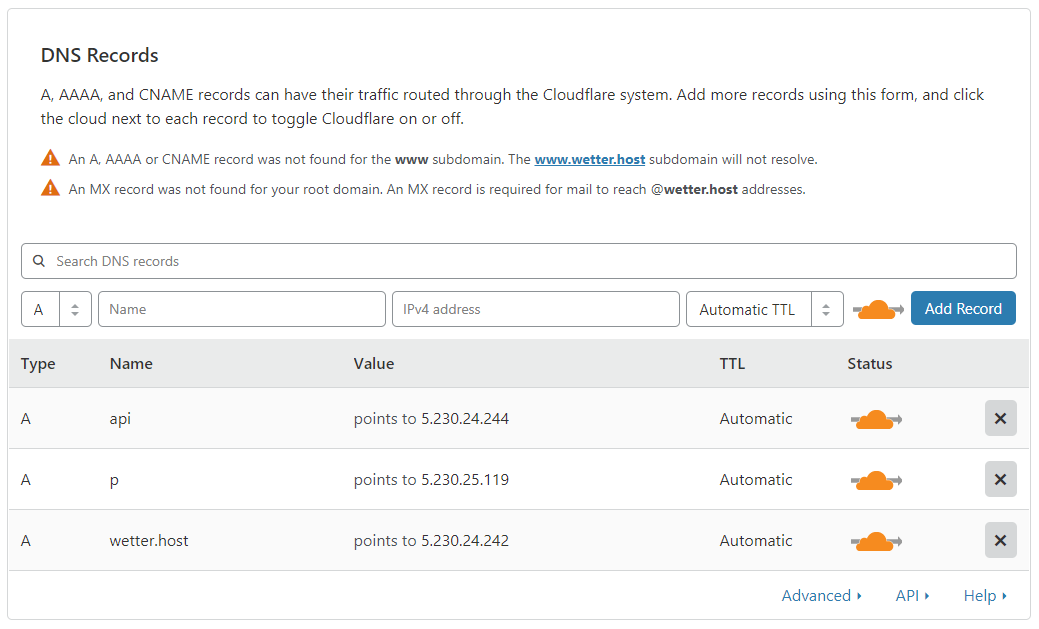
\includegraphics[height=170px]{demo2.png}\hfill
    \vspace*{10px}
	\captionof{figure}{
		\label{fig:karte2}
		\raggedright
		\textbf{\small HA traefik Beispiel}
		\\
		Quelle: Bei mir Daham, Gestan am Obend
		\vspace*{-9px}
		\\
	}   
\end{minipage}
\end{frame}

\section{Ré­su­mé}
\begin{frame}{Ré­su­mé}
	„Livedemos san a bissl risky“ - Florian Kleber
\end{frame}
%\begin{frame}[standout]
%	Danke für Eure Aufmerksamkeit
%\end{frame}


\appendix
%\begin{frame}{Quellen}
%
%  \bibliography{demo}
%  \bibliographystyle{abbrv}
%
%\end{frame}

\end{document}